\documentclass[a4paper, 12pt]{beamer}

\usetheme{CambridgeUS}
\usecolortheme{beaver}
\usefonttheme{structuresmallcapsserif}

%%%%%%%%%% Packages %%%%%%%%%%

\usepackage[slovene]{babel}
\usepackage[utf8]{inputenc}
\usepackage[T1]{fontenc}
\usepackage{lmodern}
\usepackage{units}
\usepackage{eurosym}
\usepackage{amsmath}
\usepackage{amssymb}
\usepackage{amsthm}
\usepackage{amsfonts}
\usepackage{mathtools}
\usepackage{graphicx}
\usepackage{color}
%\usepackage{url}
\usepackage{hyperref}
\usepackage{enumerate}
\usepackage{enumitem}
\usepackage{pifont}

\theoremstyle{definition} 
\newtheorem*{definicija}{Definicija}
\newtheorem*{trditev}{Trditev}


\theoremstyle{plain} 
\newtheorem*{izrek}{Izrek}
\newtheorem*{posledica}{Posledica}
\newtheorem*{zgled}{Zgled}
\newtheorem{primer}{Primer}


\definecolor{bostonuniversityred}{rgb}{0.8, 0.0, 0.0}

%%%%%%%%%%%%%%%%%%%%%%%%%%%%%%%%%%%%%%%%%%%%%%%%%%%%%%%%%%%%%%%%%%%%%%%


\title[CAGD projekt]{Krožnica in ostale stožnice \\
v racionalni B\'ezierjevi obliki
}
\author{Sara Bizjak in Urša Blažič}
\institute[FMF]{Fakulteta za matematiko in fiziko}


\begin{document}

\titlepage

%%%%%%%%%%%%%%%%%%%%%%%%%%%%%%%%%%%%%%%%%%%%%%%%%%%%%%%%%%%%%%%%%%%%%%%%%%%%%%%%%%

% SARA
\begin{frame}
\frametitle{Motivacija}
    
\begin{figure}[ht!]
    \centering
    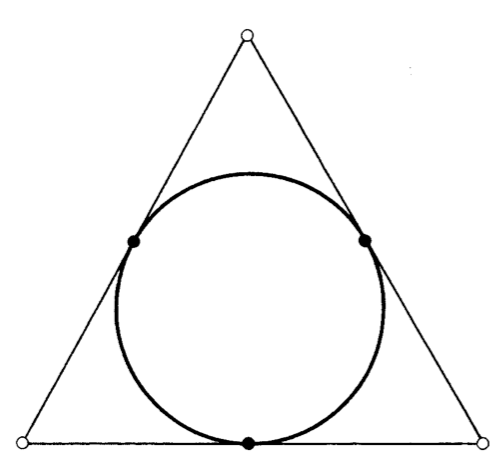
\includegraphics[width=60mm]{krog_po_delih.png}
    \caption{Krog, sestavljen iz treh racionalnih kvadratičnih B\'ezierjevih krivulj.}
    \label{slika:krogpodelih}
\end{figure}
    
    
\end{frame}

%%%%%%%%%%%%%%%%%%%%%%%%%%%%%%%%%%%%%%%%%%%%%%%%%%%%%%%%%%%%%%%%%%%%%%%%%%%%%%%%%%

% URŠA
\begin{frame}
\frametitle{Racionalna B\'ezierjeva krivulja}
    
    stopnje $n$ v $\mathbb{R}^d$ je projekcija polinomske B\'ezierjeve krivulje stopnje $n$ v $\mathbb{R}^{d+1}$ na hiperravnino $w=1$, kjer točko v  $\mathbb{R}^{d+1}$  označimo z
    $$(\boldsymbol{x},w)=(x_1,x_2,\dots,x_d,w).$$
    Projekcija je definirana kot
    $$(\boldsymbol{x},w)\mapsto (\frac{1}{w}\boldsymbol{x},1).$$

    \begin{definicija}
        \emph{Racionalna B\'ezierjeva krivulja} stopnje $n$ je podana s parametrizacijo $\boldsymbol{r}:[0,1]\rightarrow \mathbb{R}^d$, določeno s predpisom
        $$\boldsymbol{r}(t)=\frac{\sum_{i=0}^n w_i\boldsymbol{b}_iB_i^n(t)}{\sum_{i=0}^n w_iB_i^n(t)}.$$      
    \end{definicija}

\end{frame}


%%%%%%%%%%%%%%%%%%%%%%%%%%%%%%%%%%%%%%%%%%%%%%%%%%%%%%%%%%%%%%%%%%%%%%%%%%%%%%%%%%

% URŠA
\begin{frame}
\frametitle{Stožnice v racionalni B\'ezierjevi obliki}

    Za uteži velja: $ w_0 = w_2 = 1$ in $w_1 = w$.
    \\
    Stožnice lahko zapišemo v racionalni B\'ezierjevi obliki kot 
    $$\boldsymbol{r}(t)=\frac{\boldsymbol{b}_0\cdot B_0^2+w\cdot\boldsymbol{b}_1\cdot B_1^2+\boldsymbol{b}_2\cdot B_2^2}{ B_0^2+w\cdot B_1^2+ B_2^2},\,\,\, t\in[0,1].$$

    \begin{figure}[ht!]
        \centering
        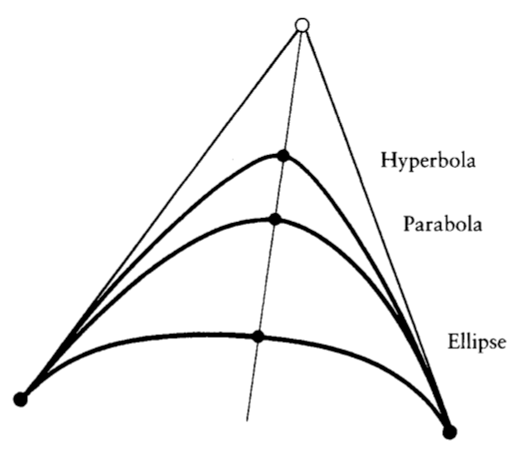
\includegraphics[width=50mm]{tri_oblike.png}
    \end{figure}
\end{frame}


%%%%%%%%%%%%%%%%%%%%%%%%%%%%%%%%%%%%%%%%%%%%%%%%%%%%%%%%%%%%%%%%%%%%%%%%%%%%%%%%%%

% SARA
\begin{frame}
\frametitle{Krožnica v racionalni B\'ezierjevi obliki}

Krožnico lahko opišemo kot racionalno B\'ezierjevo krivuljo 
$$\boldsymbol{C}(t)=(X(t),Y(t))$$ 
s pomočjo projekcije krivulje 
$$\boldsymbol{\tilde{C}}(t)=(\tilde{X}(t), \tilde{Y(t)}, W(t))$$ 
na ravnino $w=1$. 

$$\tilde{X}(t)^2+\tilde{Y}(t)^2-W(t)^2=0$$

\end{frame}


%%%%%%%%%%%%%%%%%%%%%%%%%%%%%%%%%%%%%%%%%%%%%%%%%%%%%%%%%%%%%%%%%%%%%%%%%%%%%%%%%%

% SARA
\begin{frame}
\frametitle{Krožnica v racionalni B\'ezierjevi obliki}
    
\begin{figure}[ht!]
    \begin{minipage}{0.5\textwidth}
        \centering
        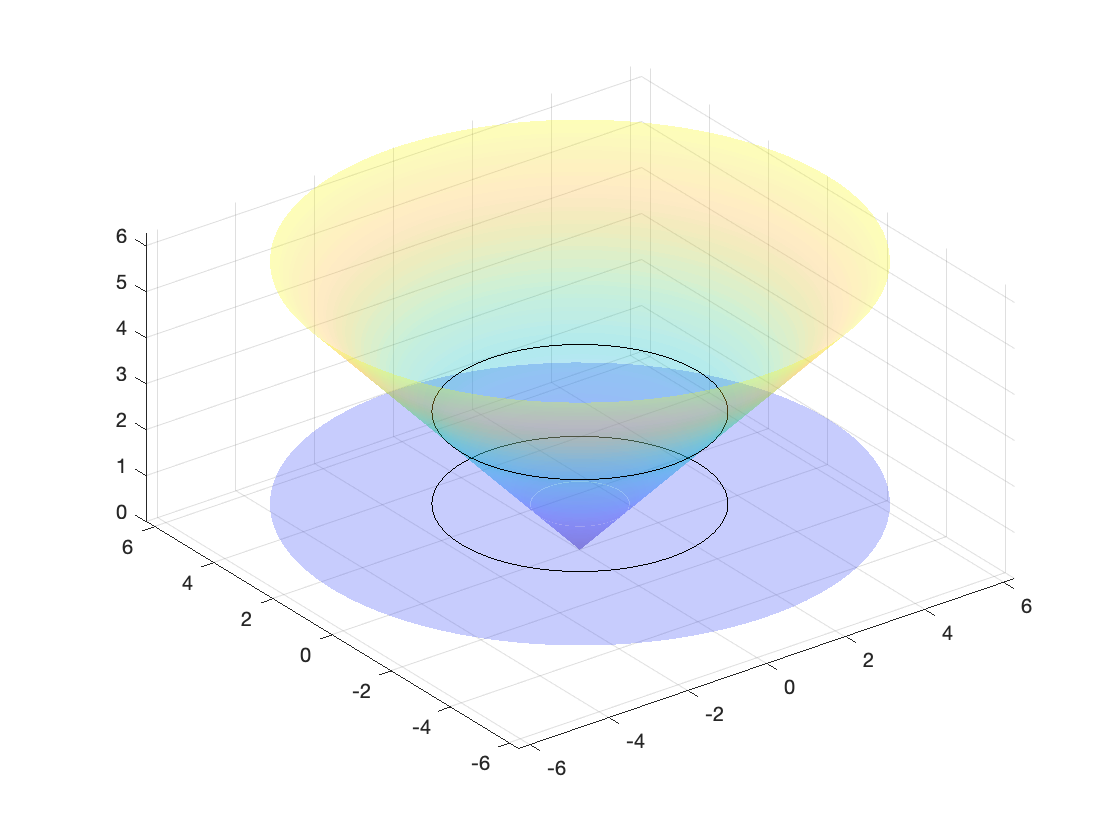
\includegraphics[width=50mm]{stozec.png}
    \end{minipage}\hfill
    \begin{minipage}{0.5\textwidth}
        \centering
        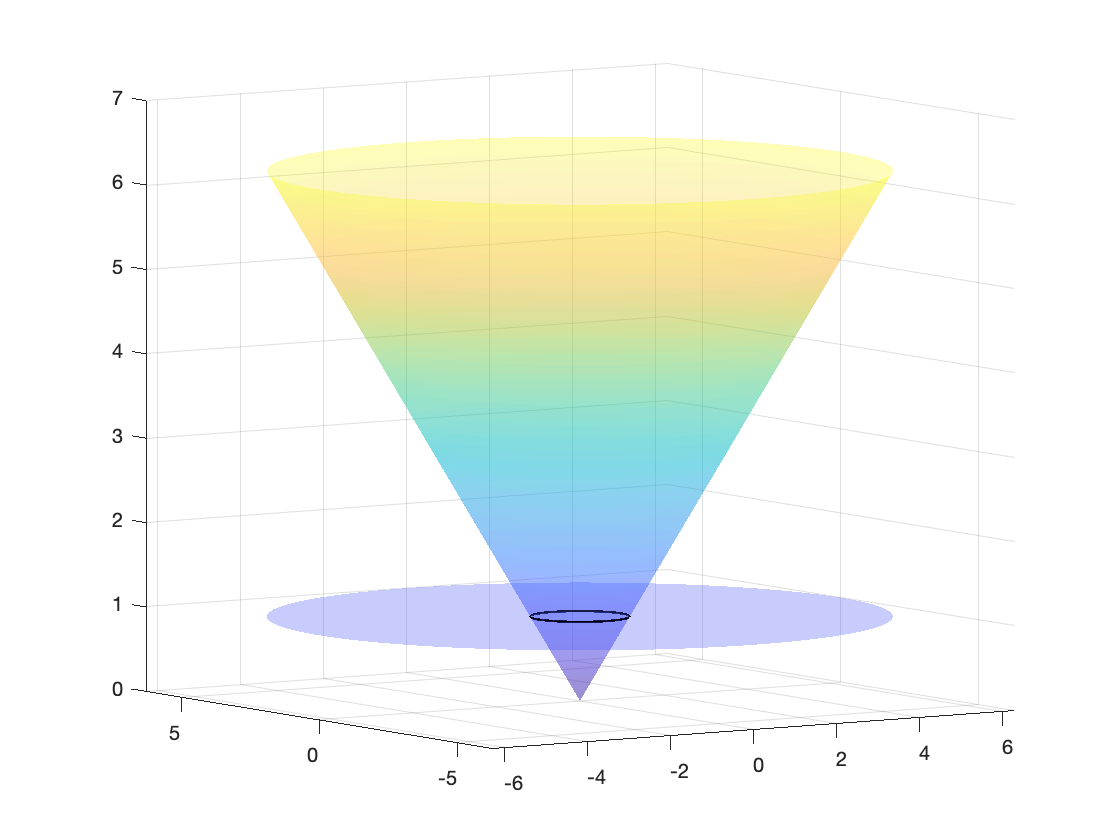
\includegraphics[width=50mm]{stozec_1.png}
    \end{minipage}\hfill
    \caption{Krožnico lahko dobimo kot projekcijo krivulje, ki leži na stožcu, na ravnino $w = 1$.}
\end{figure}

\end{frame}
    
    
%%%%%%%%%%%%%%%%%%%%%%%%%%%%%%%%%%%%%%%%%%%%%%%%%%%%%%%%%%%%%%%%%%%%%%%%%%%%%%%%%%

% SARA
\begin{frame}
\frametitle{Kvadratična krivulja}
    
\begin{figure}[ht!]
    \begin{minipage}{0.5\textwidth}
        \centering
        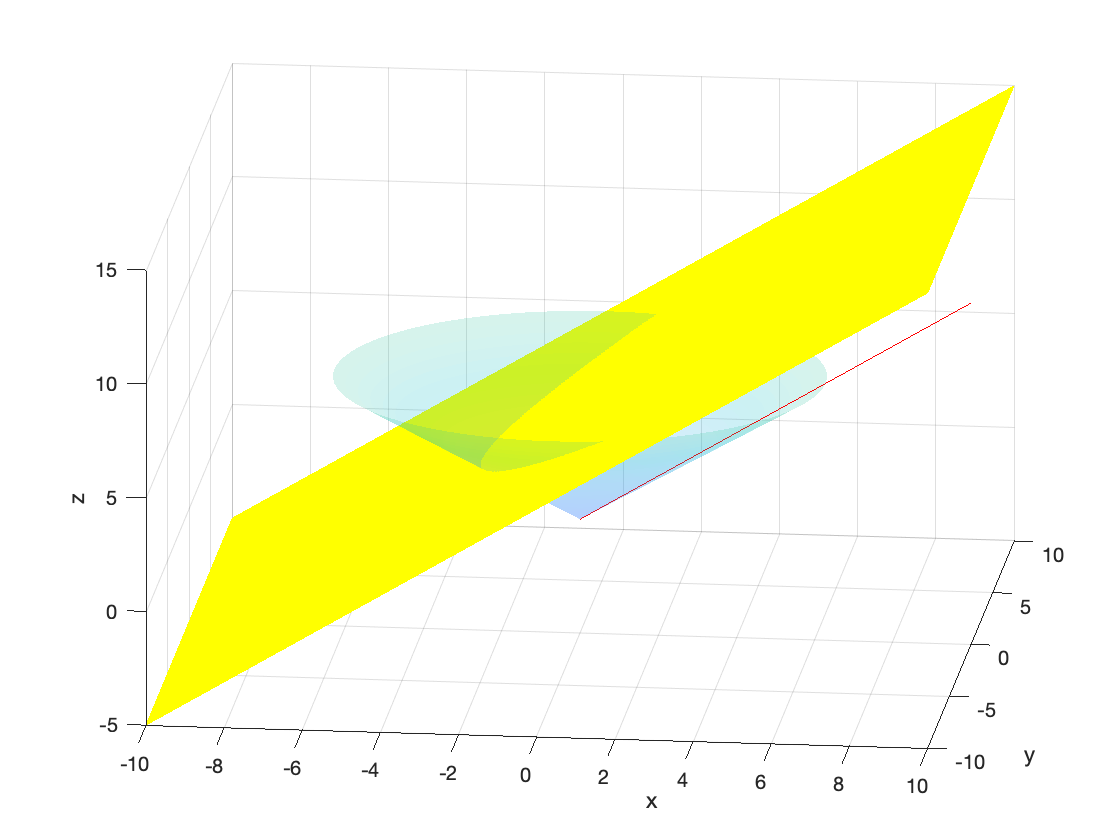
\includegraphics[width=60mm]{stozec_presek_1.png}
    \end{minipage}\hfill
    \begin{minipage}{0.5\textwidth}
        \centering
        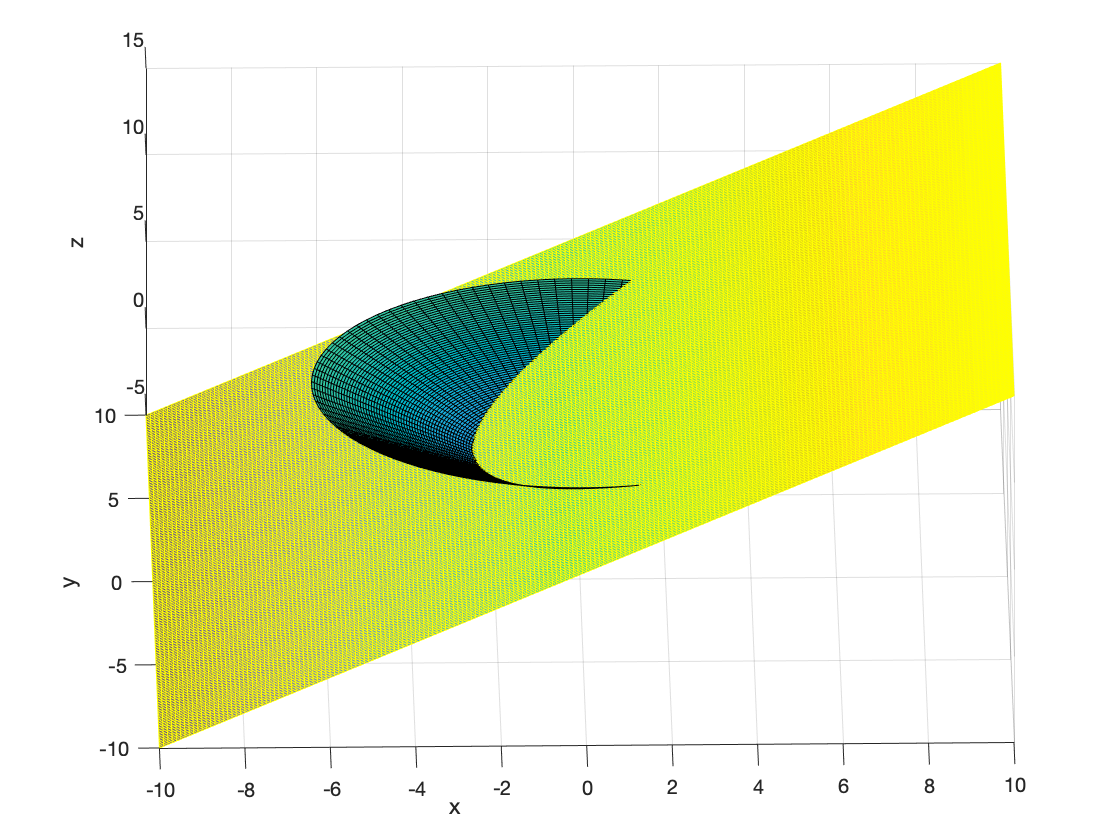
\includegraphics[width=60mm]{stozec_presek_2.png}
    \end{minipage}\hfill
    \caption{Presek stožca z ravnino, ki je vzporedna njegovi nosilki. Na sliki je ravnina obarvana z rumeno barvo, nosilka pa z rdečo.}
\end{figure}
    
\end{frame}
    
    
%%%%%%%%%%%%%%%%%%%%%%%%%%%%%%%%%%%%%%%%%%%%%%%%%%%%%%%%%%%%%%%%%%%%%%%%%%%%%%%%%%

% SARA
\begin{frame}
\frametitle{Kvadratična krivulja}
    
    S parabolo lahko zapišemo krožne loke, ki jih opišemo z naslednjim kontrolnim poligonom:
    \begin{align*}
        \boldsymbol{\tilde{b}}_0 &= (\cos{\theta}, -\sin{\theta}, 1)\\
        \boldsymbol{\tilde{b}}_1 &= (1, 0, \cos{\theta})\\
        \boldsymbol{\tilde{b}}_2 &= (\cos \theta, \sin\theta, 1),
    \end{align*}
    kjer je $\theta$ polovični kot krožnega loka. 

    
\end{frame}
    
    
%%%%%%%%%%%%%%%%%%%%%%%%%%%%%%%%%%%%%%%%%%%%%%%%%%%%%%%%%%%%%%%%%%%%%%%%%%%%%%%%%%

% SARA
\begin{frame}
    \frametitle{Kubična krivulja}
    
    \begin{figure}[ht!]
        \begin{minipage}{0.5\textwidth}
            \centering
            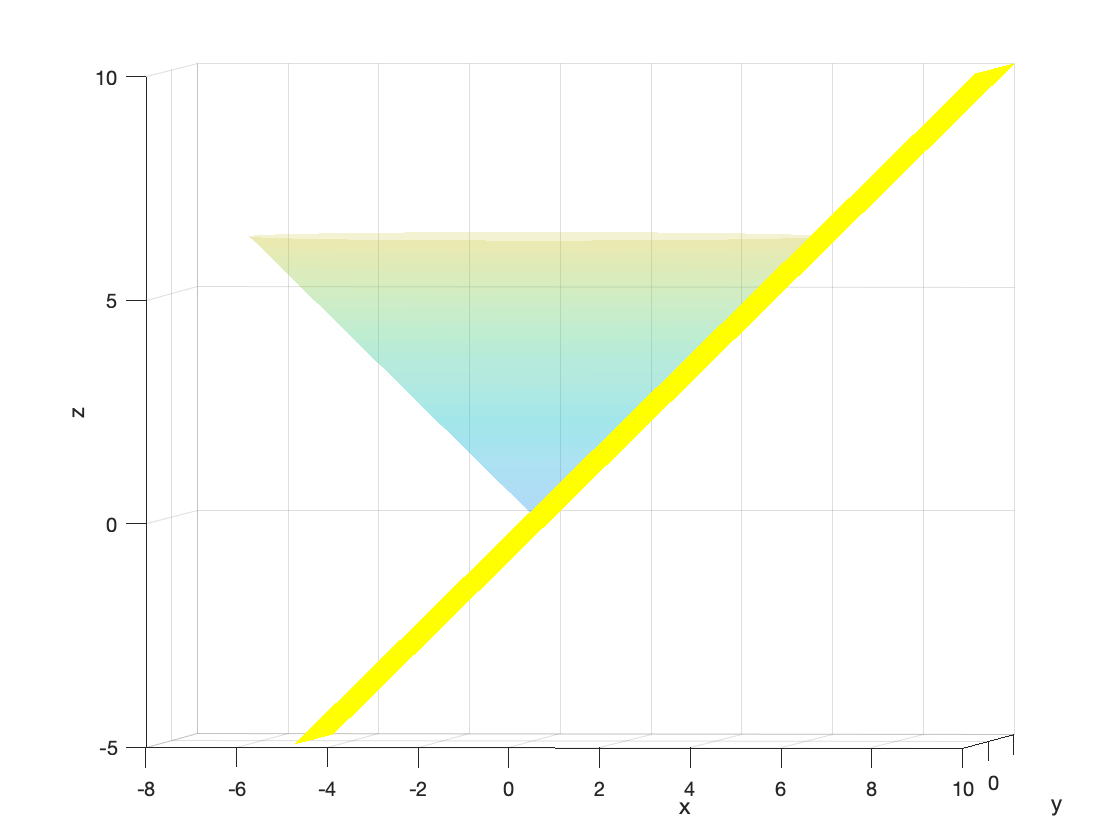
\includegraphics[width=60mm]{stozec_tang_1.png}
        \end{minipage}\hfill
        \begin{minipage}{0.5\textwidth}
            \centering
            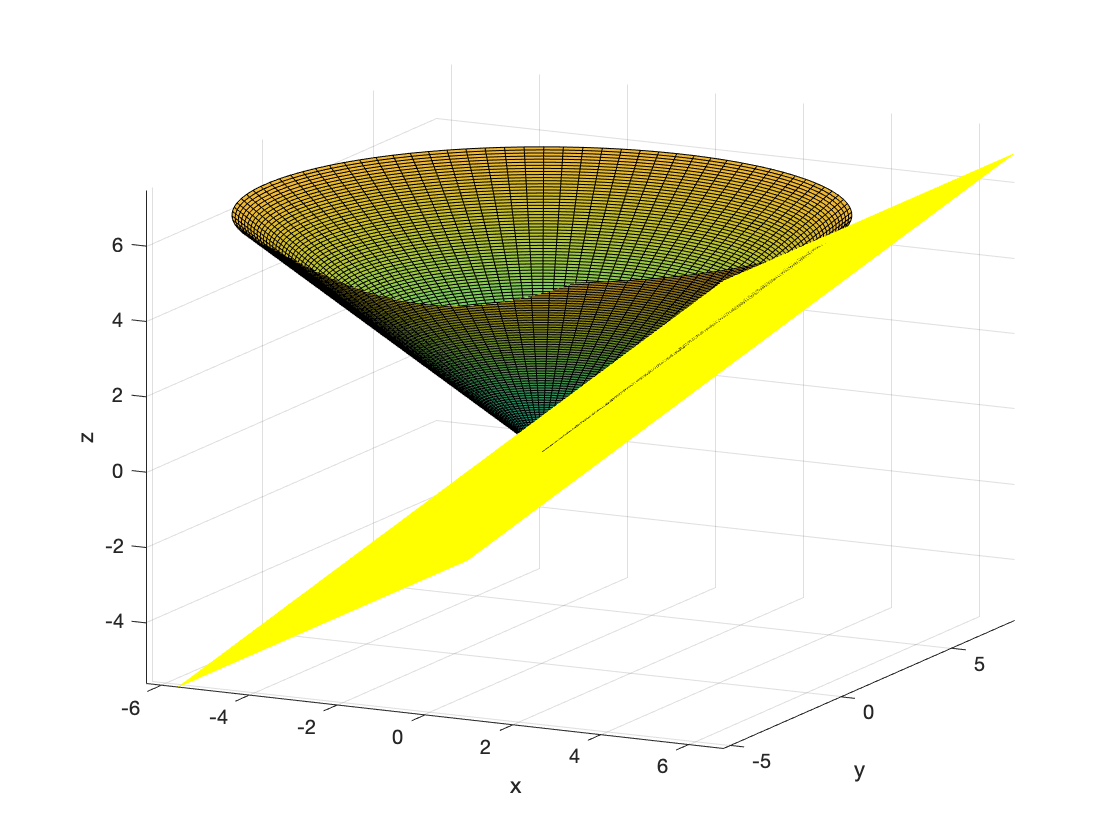
\includegraphics[width=60mm]{stozec_tang_2.png}
        \end{minipage}\hfill
        \caption{Presek stožca s tangentno ravnino. Presek je premica, ki je enaka eni od nosilk stožca.}
    \end{figure}

    
\end{frame}
    
    
%%%%%%%%%%%%%%%%%%%%%%%%%%%%%%%%%%%%%%%%%%%%%%%%%%%%%%%%%%%%%%%%%%%%%%%%%%%%%%%%%%

% SARA
\begin{frame}
\frametitle{Krivulja 4. stopnje}
    Enačbe:

        \begin{align*}
            \tilde{y}_3 &=- \tilde{y}_1 \\
            \tilde{x}_3 &= - \tilde{x}_1 \\
            3\tilde{x}_2 + 4\tilde{y}_1^2 - 3w_2 &= 0 \\
            \tilde{x}_1\tilde{x}_2 + \tilde{y}_1\tilde{y}_2  - \tilde{x}_1w_2 &= 0 \\
            9\tilde{x}_2^2 - 8\tilde{y}_1^2 + 9\tilde{y}_2^2 - 9w_2^2&= 0 
        \end{align*}
\end{frame}
    
    
%%%%%%%%%%%%%%%%%%%%%%%%%%%%%%%%%%%%%%%%%%%%%%%%%%%%%%%%%%%%%%%%%%%%%%%%%%%%%%%%%%

% SARA
\begin{frame}
\frametitle{Krivulja 4. stopnje} 
    Kontrolne točke:
 
        \begin{align*}
            \boldsymbol{\tilde{b}}_0 &= (1,0,1) \\
            \boldsymbol{\tilde{b}}_1 &= (\tilde{x}_1,\pm\alpha,\tilde{x}_1) \\
            \boldsymbol{\tilde{b}}_2 &= (-\frac{3w_2-4\tilde{x}_1^2+2}{3},\pm\frac{4}{3}\tilde{x}_1\alpha,w_2) \\
            \boldsymbol{\tilde{b}}_3 &= (-\tilde{x}_1,\mp\alpha,-\tilde{x}_1) \\
            \boldsymbol{\tilde{b}}_4 &= (1,0,1)
        \end{align*}
    
        kjer je $\alpha=(\frac{3w_2}{2}-\tilde{x}_1^2+\frac{1}{2})^{\frac{1}{2}}$
   
   
\end{frame}

%%%%%%%%%%%%%%%%%%%%%%%%%%%%%%%%%%%%%%%%%%%%%%%%%%%%%%%%%%%%%%%%%%%%%%%%%%%%%%%%%%

% SARA
\begin{frame}
\frametitle{Krivulja 4. stopnje}
    Kontrolne točka za $\tilde{x}_1=0$:

        \begin{align*}
            \boldsymbol{\tilde{b}}_0 &= (1,0,1) \\
            \boldsymbol{\tilde{b}}_1 &= (0,\pm (\frac{1}{2}+\frac{3}{2}w_2)^{1/2},0) \\
            \boldsymbol{\tilde{b}}_2 &= (-\frac{2}{3}-w_2,0,w_2) \\
            \boldsymbol{\tilde{b}}_3 &= (0,\mp(\frac{1}{2}+\frac{3}{2}w_2)^{1/2},0) \\
            \boldsymbol{\tilde{b}}_4 &= (1,0,1)
        \end{align*}
  
    
\end{frame}
    
    
%%%%%%%%%%%%%%%%%%%%%%%%%%%%%%%%%%%%%%%%%%%%%%%%%%%%%%%%%%%%%%%%%%%%%%%%%%%%%%%%%%

% URŠA
\begin{frame}
    \frametitle{Kubični B\'ezierjevi loki}
    \begin{align*}
        w_1 = \tilde{x_1}\cos{\theta} - \tilde{y_1} \sin{\theta}   \\
        w_2 = \tilde{x_2}\cos{\theta} + \tilde{y_2} \sin{\theta}   \\
        3\tilde{x_1}^2\sin^2{\theta} + 3\tilde{y_1}^2\cos^2{\theta} - 4\tilde{y_2} \sin{\theta}  + 6\tilde{x_1}\tilde{y_1} \sin{\theta} \cos{\theta} = 0 \\
        9\tilde{x_1}\tilde{x_2}\sin^2{\theta} + 9\tilde{y_1}\tilde{x_2}\cos{\theta} \sin{\theta} - 9\tilde{x_1} \tilde{y_2} \cos{\theta} \sin{\theta}+ \\
        + 9 (1 + \sin^2{\theta}) \tilde{y_1} \tilde{y_2} - 2\sin^2{\theta} = 0 \\
        3\tilde{x_2}^2 \sin^2{\theta}+ 3\tilde{y_2}^2 \cos^2{\theta}+ 4\tilde{y_1} \sin{\theta}  - 6\tilde{x_2}\tilde{y_2}\sin{\theta} \cos{\theta}  = 0 
    \end{align*}
        

\end{frame}

%%%%%%%%%%%%%%%%%%%%%%%%%%%%%%%%%%%%%%%%%%%%%%%%%%%%%%%%%%%%%%%%%%%%%%%%%%%%%%%%%%
%%%%%%%%%%%%%%%%%%%%%%%%%%%%%%%%%%%%%%%%%%%%%%%%%%%%%%%%%%%%%%%%%%%%%%%%%%%%%%%%%%

% URŠA
\begin{frame}
    Edini možni kubični B\'ezierjevi krožni loki so oblike
    $$\boldsymbol{C}(t)=\frac{(\tilde{X}(t),\tilde{Y}(t))(aB_0^1(t)+bB_1^1(t))}{W(t)(aB_0^1(t)+bB_1^1(t))},$$
    kjer je $$\frac{(\tilde{X}(t),\tilde{Y}(t))}{W(t)}$$
    kvadratični krožni lok.
    Za kontrolni poligon kvadratičnega krožnega loka izberemo
    \begin{align*}
    \boldsymbol{\tilde{b}}_0 &= (\cos{\theta}, -\sin{\theta}, 1)\\
    \boldsymbol{\tilde{b}}_1 &= (\sqrt{w_2}, 0,\sqrt{w_2} \cos{\theta})\\
    \boldsymbol{\tilde{b}}_2 &= (w_2\cos \theta, w_2 \sin\theta, w_2),
    \end{align*}
    kjer je $\theta$ polovični kot krožnega loka. 

\end{frame}

%%%%%%%%%%%%%%%%%%%%%%%%%%%%%%%%%%%%%%%%%%%%%%%%%%%%%%%%%%%%%%%%%%%%%%%%%%%%%%%%%%

% URŠA
\begin{frame}
Kontrolne točke kubičnega B\'ezierjevega krožnega loka:
\begin{align*}
\boldsymbol{\tilde{b}}_0 &= (\cos{\theta}, -\sin{\theta}, 1)\\
\boldsymbol{\tilde{b}}_1 &= \left ( \left (\frac{2}{3\sqrt{b}}+\frac{b\cos \theta}{3}\right ),-\frac{b \sin \theta}{3},\left (\frac{2\cos \theta}{3\sqrt{b}}+\frac{b}{3}\right )\right )\\
\boldsymbol{\tilde{b}}_2 &= \left ( \left (\frac{\cos \theta}{3b}+\frac{2\sqrt{b}}{3}\right ),\frac{\sin \theta}{3b},\left (\frac{2\sqrt{b}\cos \theta}{3}+\frac{1}{3b}\right )\right )\\
\boldsymbol{\tilde{b}}_3 &= (\cos \theta, \sin\theta, 1),
\end{align*}
Nenegativne uteži:
$$\cos \theta \geq -\frac{b^{3/2}}{2}\quad\text{ in }\quad \cos  \theta \geq -\frac{1}{2b^{3/2}}$$
\end{frame}

\end{document}